%mainfile: Multimodal_learning.tex
\title[Multimodal Learning]
      {Multimodal Learning:\\
       A case study for Gesture and Audio-Visual Speech Recognition}
\author{Yu-Guan Hsieh}
\date{September 2017}


\begin{frame}
  \begin{textblock*}{2.2cm}(10.4cm,0.5cm) % {block width} (coords)
  
\includegraphics[width=2.2cm]{slides/ens}
  \end{textblock*}
  \begin{textblock*}{4cm}(0.3cm,8.2cm) % {block width} (coords)
  
\includegraphics[width=4cm]{slides/logo_behaviorsai}
  \end{textblock*}
  \flushleft
  {\LARGE \color{BlueViolet} Soutenance de Stage de L3\\}
  \vspace{0.5em}
  {\Large \color{Blue} Multimodal Learning:\\}
  {\Large \color{Blue}
    A case study for Gesture and Audio-Visual Speech Recognition\\}
  \vspace{1.7em}
  \flushright
  {\large Hsieh Yu-Guan (Info 2016)\\}
  \vspace{0.7em}
  {\large Supervised by\\}
  {\large Amélie Cordier \& Mathieu Lefort\\}
  \vspace{0.7em}
  {\large Internship period:
    $14^{\mathrm{th}}$ June 2017 -- $11^{\mathrm{th}}$ August 2017\\}
\end{frame}

\section{Introduction}

\begin{frame}
  \frametitle{Introduction}
  \begin{itemize}
    \item BEHAVIORS.AI
    \item Hoomano \& LIRIS
    \item TensorFlow
  \end{itemize}
  \begin{center}
    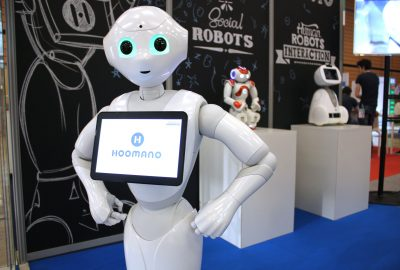
\includegraphics[width=0.6\linewidth]{slides/pepper}
  \end{center}
\end{frame}

\begin{frame}
  \frametitle{Introduction}
  \begin{itemize}[<+->]
    \item Artifical Intelligence
    \item > Robotics (embodied paradigme)
    \item > Developmental robotics
    \item > Multimodal learning
    \item > Gesture and Audio-Visual recogntion
  \end{itemize}
\end{frame}

\section{Deep Network Architectures}

\subsection{CNN}

\begin{frame}
  \frametitle{Deep Network Architectures -- Convolutional
    Neural Networks (CNNs)}
  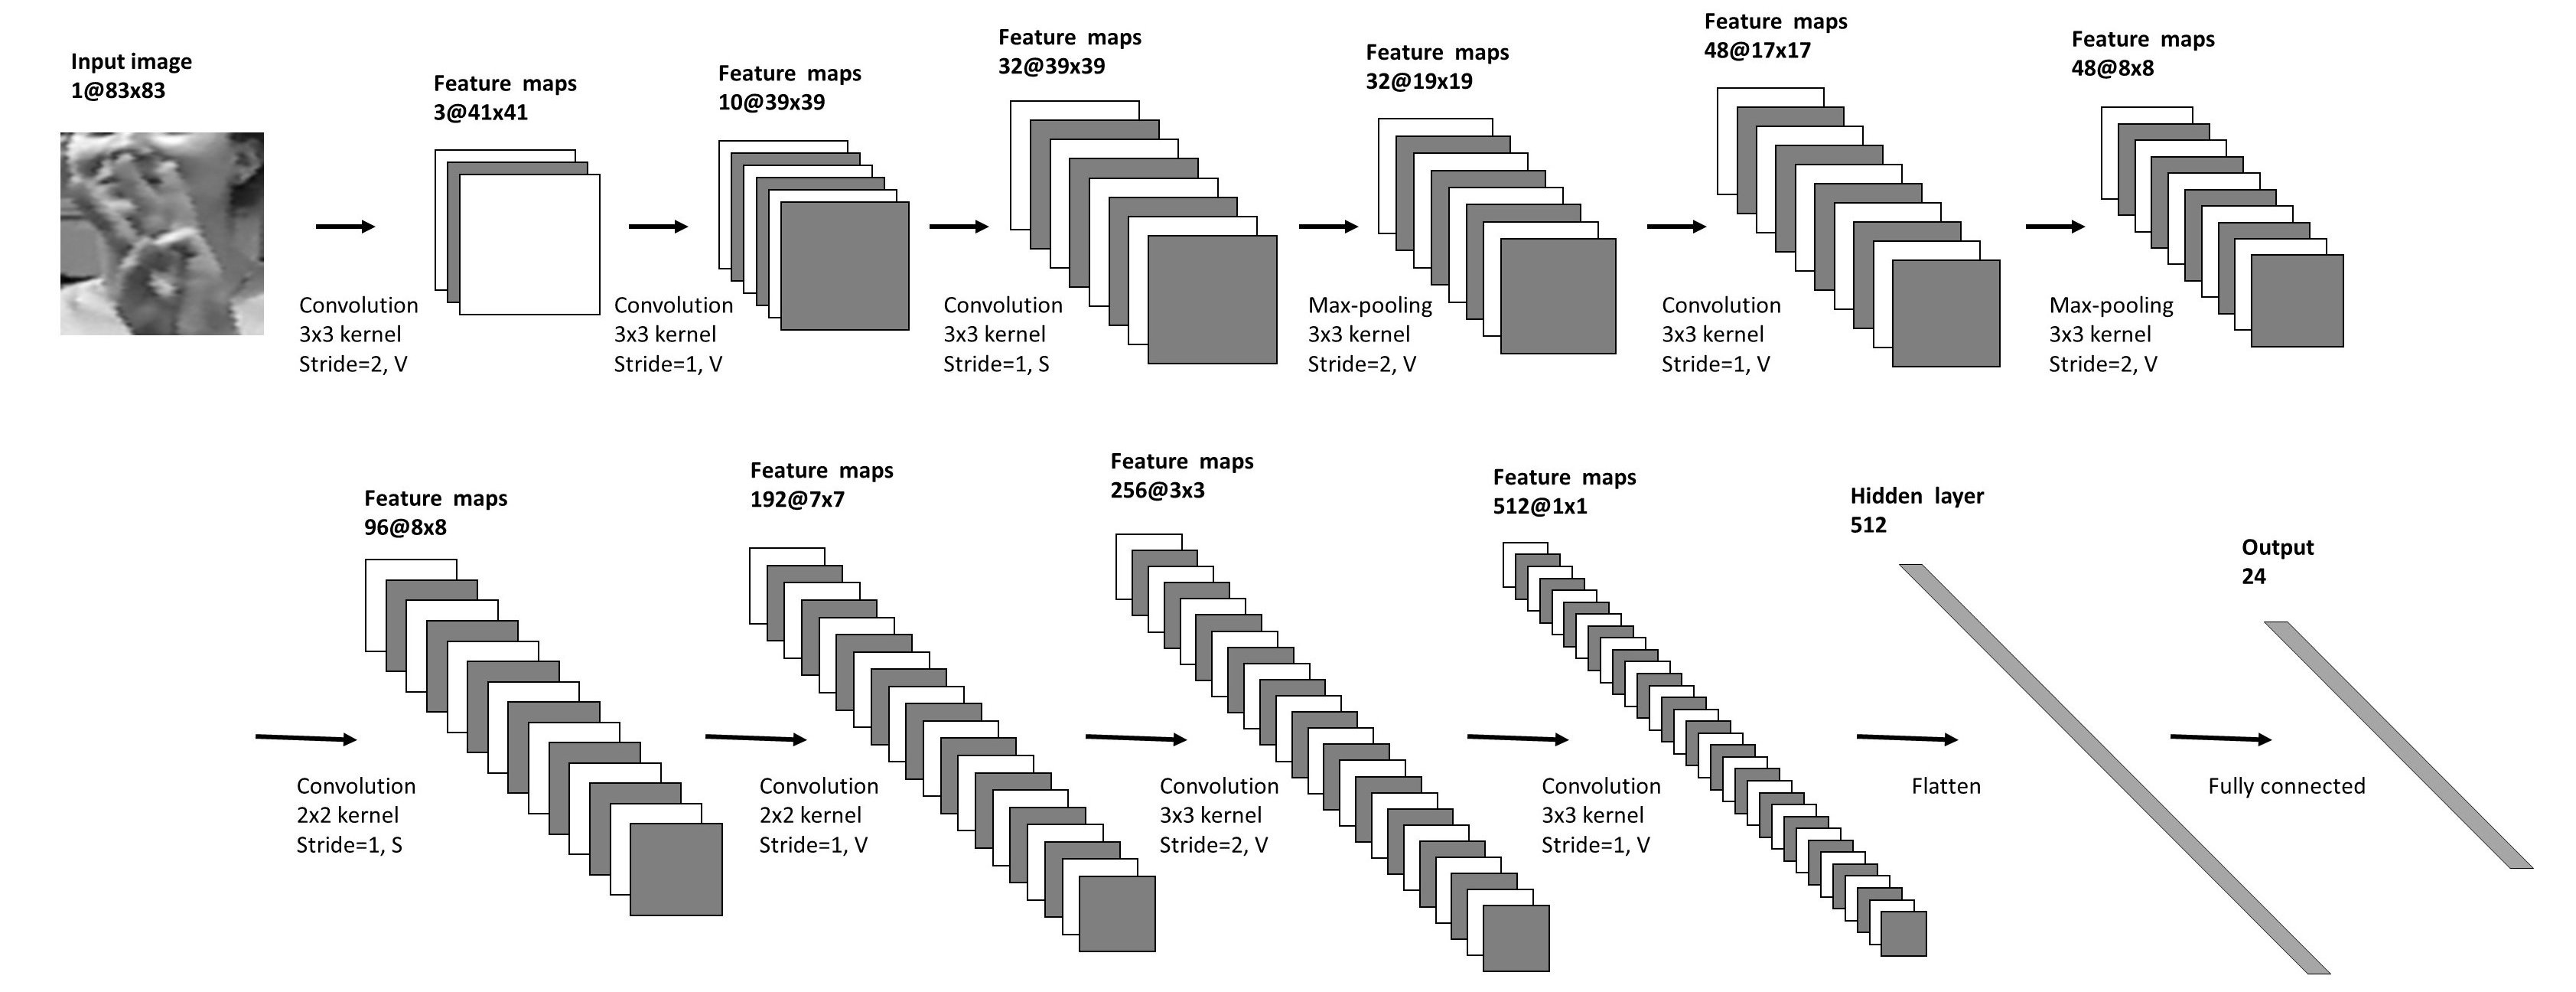
\includegraphics[width=0.94\paperwidth]{slides/CNN10}
\end{frame}

\begin{frame}
\frametitle{Deep Network Architectures -- Convolutional
  Neural Networks (CNNs) -- Convolution}
  \vspace*{1.2em}
  \centering
  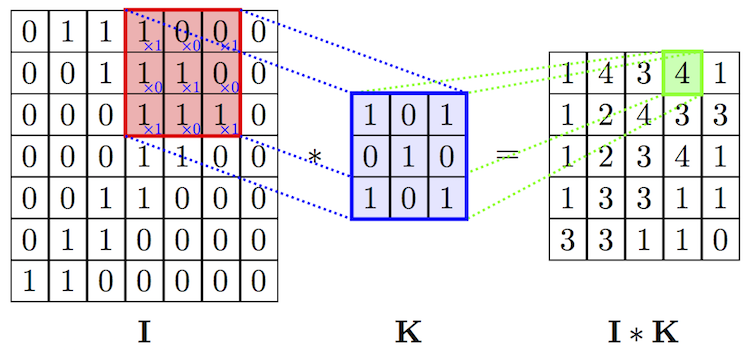
\includegraphics[width=0.8\linewidth]{slides/convolution}\\
  \vspace*{-0.4em}
  \flushleft
  Source: 
    \href{https://cambridgespark.com/content/tutorials/convolutional-neural-networks-with-keras/index.html}
    {https://cambridgespark.com/content/tutorials/convolutional-neural-networks-with-keras/index.html}\\
  Also see \href{https://github.com/vdumoulin/conv\_arithmetic}
    {https://github.com/vdumoulin/conv\_arithmetic}
\end{frame}

\begin{frame}
\frametitle{Deep Network Architectures -- Convolutional
  Neural Networks (CNNs) -- Max-pooling}
  \vspace*{0.6em}
  \centering
  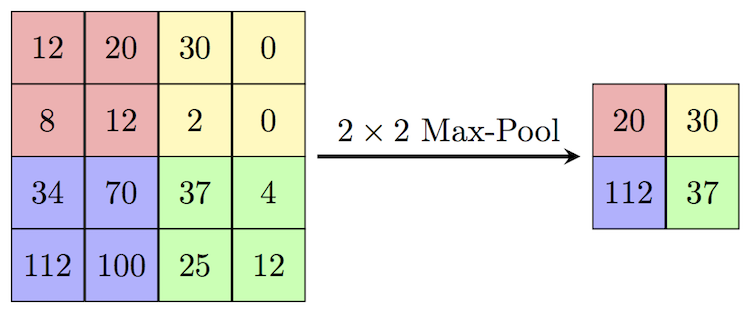
\includegraphics[width=0.6\linewidth]{slides/pooling}\\
  \vspace*{0.6em}
  \flushleft
  Source: 
    \href{https://cambridgespark.com/content/tutorials/convolutional-neural-networks-with-keras/index.html}
    {https://cambridgespark.com/content/tutorials/convolutional-neural-networks-with-keras/index.html}\\
\end{frame}

\subsection{Autoencoder}

\begin{frame}
\frametitle{Deep Network Architectures -- Autoencoder}
  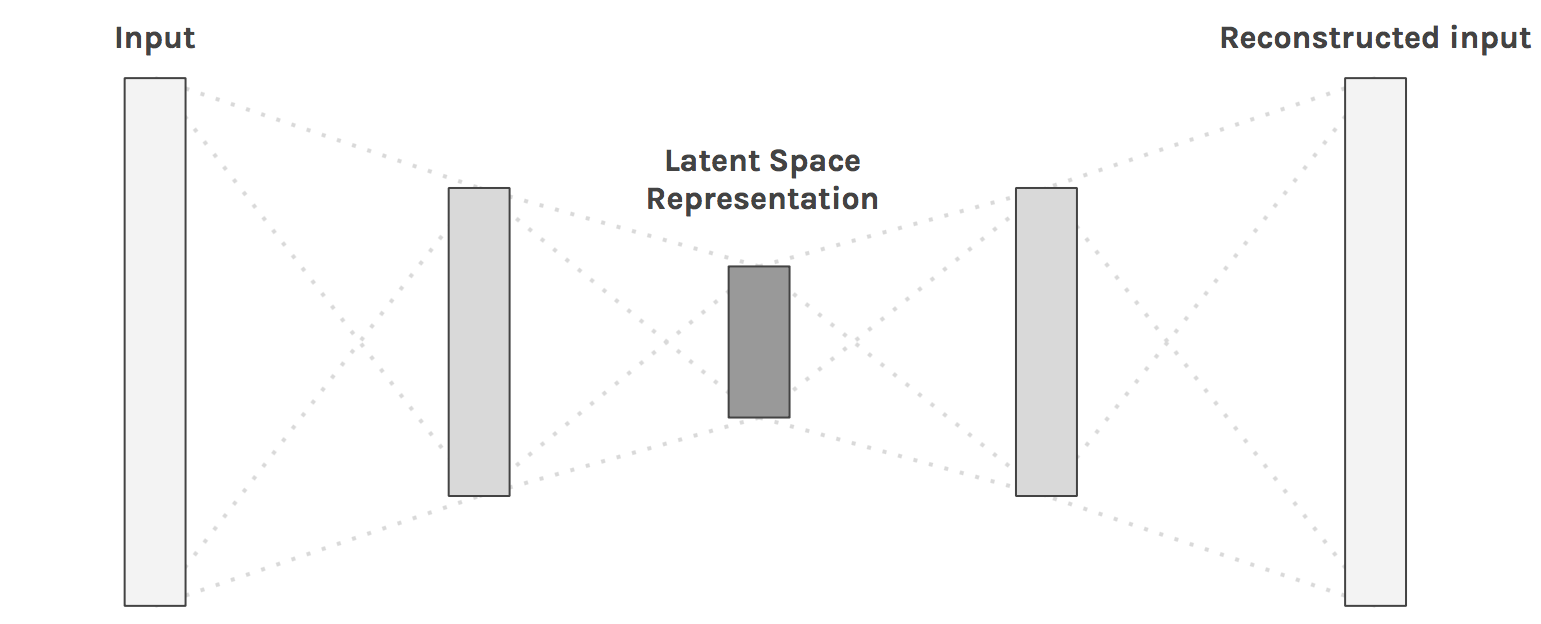
\includegraphics[width=\linewidth]{slides/autoencoder}\\
  \vspace*{1em}
  Source:
    \href{https://hackernoon.com/autoencoders-deep-learning-bits-1-11731e200694}
    {https://hackernoon.com/autoencoders-deep-learning-bits-1-11731e200694}
\end{frame}

\subsection{CAE}

\begin{frame}
\frametitle{Deep Network Architectures -- Convolutional Autoencoder}
  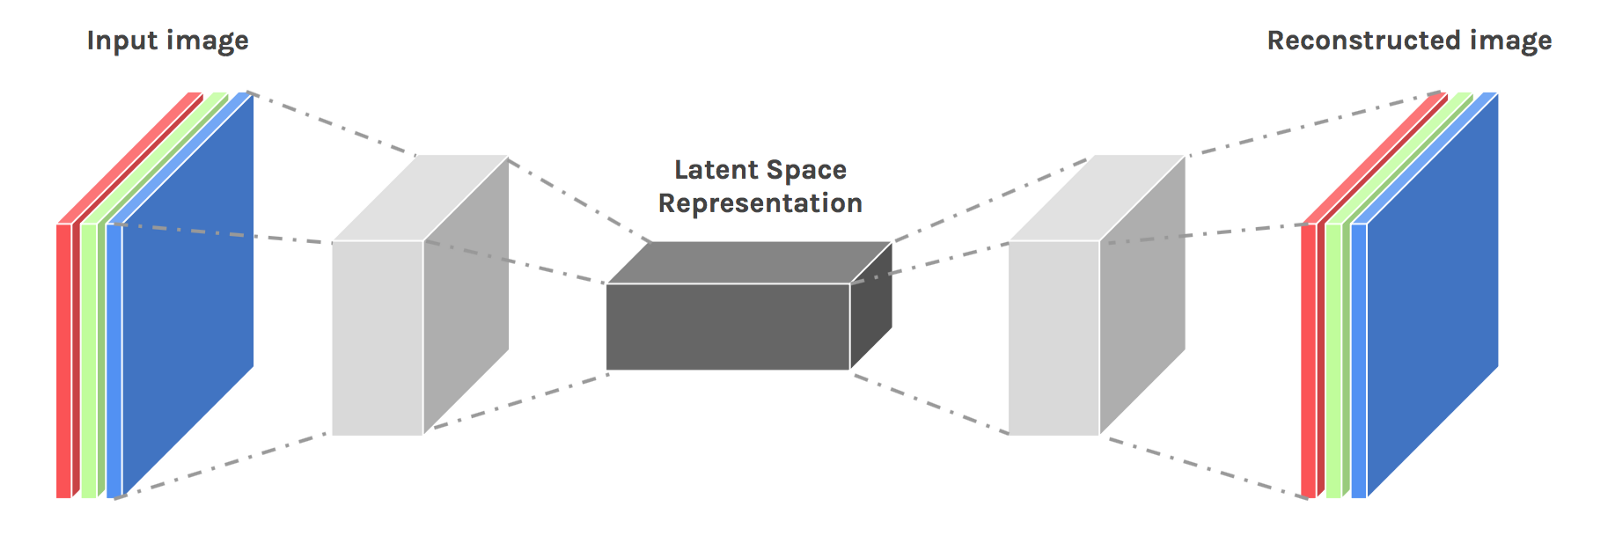
\includegraphics[width=\linewidth]{slides/CAE}\\
  \vspace*{1em}
  Source:
    \href{https://hackernoon.com/autoencoders-deep-learning-bits-1-11731e200694}
    {https://hackernoon.com/autoencoders-deep-learning-bits-1-11731e200694}
\end{frame}

\subsection{Training a Machine Learning Model}

\begin{frame}
\frametitle{Training a Machine Learning Model}
  \begin{itemize}
    \item Loss function: cross-entropy, L2-distance
    \item Stochastic gradient descent (SGD)
    \item Backpropagation
    \item Varaints of SGD: AdaGrad, Adam
  \end{itemize}
\end{frame}

\section{Datasets}

\subsection{ASL Finger Spelling}

\begin{frame}
\frametitle{Datasets -- ASL Finger Spelling}
  \begin{itemize}
    \item RGB and depth
    \item More than 60000 images for each modality
    \item 24 static signs in American Sign Language
    \item 5 subjects
    \item Only one channel in input
    \item Resized to $83 \times 83$ and Z-normalization
  \end{itemize}
  \begin{figure}[H]
    \centering
    \hfill
    %
    \begin{subfigure}{0.21\linewidth}
      \centering
      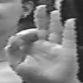
\includegraphics[width=\linewidth]{%
        dataset/fingerspelling5/exs/st/g1}
      \caption{}
    \end{subfigure}
    %
    \hfill
    %
    \begin{subfigure}{0.21\linewidth}
      \centering
      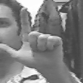
\includegraphics[width=\linewidth]{%
        dataset/fingerspelling5/exs/st/g2}
      \caption{}
    \end{subfigure}
    %
    \hfill
    %
    \begin{subfigure}{0.21\linewidth}
      \centering
      
\includegraphics[width=\linewidth]{%
        dataset/fingerspelling5/exs/st/d1}
      \caption{}
    \end{subfigure}
    %
    \hfill
    %
    \begin{subfigure}{0.21\linewidth}
      \centering
      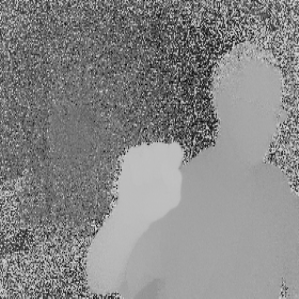
\includegraphics[width=\linewidth]{%
        dataset/fingerspelling5/exs/st/d2}
      \caption{}
    \end{subfigure}
    %
  \end{figure}
\end{frame}

\subsection{AVLetters}

\begin{frame}
\frametitle{Datasets -- AVLetters}
  \begin{itemize}
    \item Audio-visual
    \item 26 letters from A to Z
    \item 10 speakers, each letter 3 times each
    \item Audio: 24 frames in input, 26 MFCCs for each frame 
    \item Video: 12 frames in input, z-normalized
  \end{itemize}
  \begin{figure}[H]
    \centering
    \hfill
    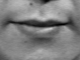
\includegraphics[width=0.15\linewidth]{%
      dataset/avletters/lips_no_data_aug/1}
    \hfill
    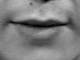
\includegraphics[width=0.15\linewidth]{%
      dataset/avletters/lips_no_data_aug/2}
    \hfill
    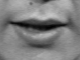
\includegraphics[width=0.15\linewidth]{%
      dataset/avletters/lips_no_data_aug/3}
    \hfill
    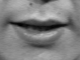
\includegraphics[width=0.15\linewidth]{%
      dataset/avletters/lips_no_data_aug/4}
    \hfill
    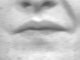
\includegraphics[width=0.15\linewidth]{%
      dataset/avletters/lips_no_data_aug/5}
    \hfill
    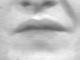
\includegraphics[width=0.15\linewidth]{%
      dataset/avletters/lips_no_data_aug/6}\\[0.15em]
    \hfill
    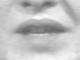
\includegraphics[width=0.15\linewidth]{%
      dataset/avletters/lips_no_data_aug/7}
    \hfill
    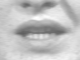
\includegraphics[width=0.15\linewidth]{%
      dataset/avletters/lips_no_data_aug/8}
    \hfill
    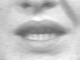
\includegraphics[width=0.15\linewidth]{%
      dataset/avletters/lips_no_data_aug/9}
    \hfill
    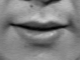
\includegraphics[width=0.15\linewidth]{%
      dataset/avletters/lips_no_data_aug/10}
    \hfill
    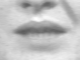
\includegraphics[width=0.15\linewidth]{%
      dataset/avletters/lips_no_data_aug/11}
    \hfill
    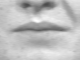
\includegraphics[width=0.15\linewidth]{%
      dataset/avletters/lips_no_data_aug/12}
    \hfill
  \end{figure}
\end{frame}

\section{Results}

\subsection{Unsupervised Learning with CAE}

\begin{frame}
\frametitle{Results -- Unsupervised Learning with CAE}
  \begin{figure}
    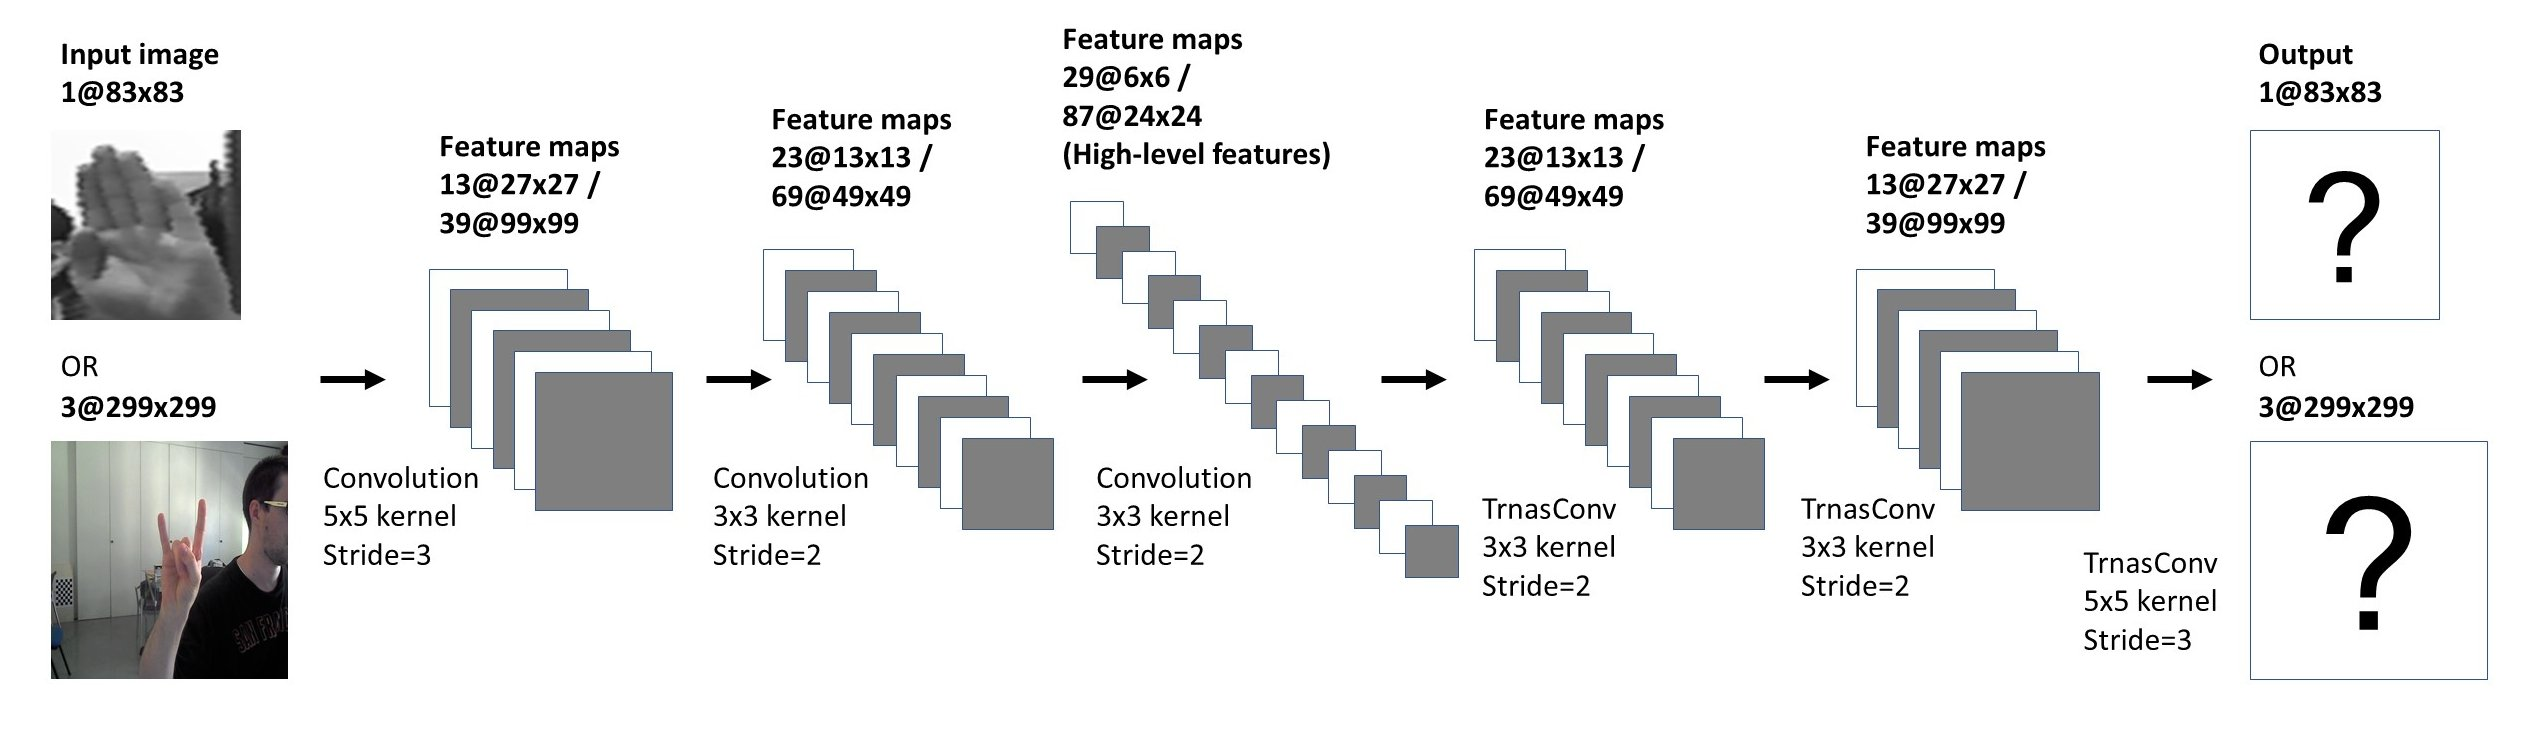
\includegraphics[width=\linewidth]{slides/CAE5}
  \end{figure}
\end{frame}

\begin{frame}
\frametitle{Results -- Unsupervised Learning with CAE}
  \begin{figure}
    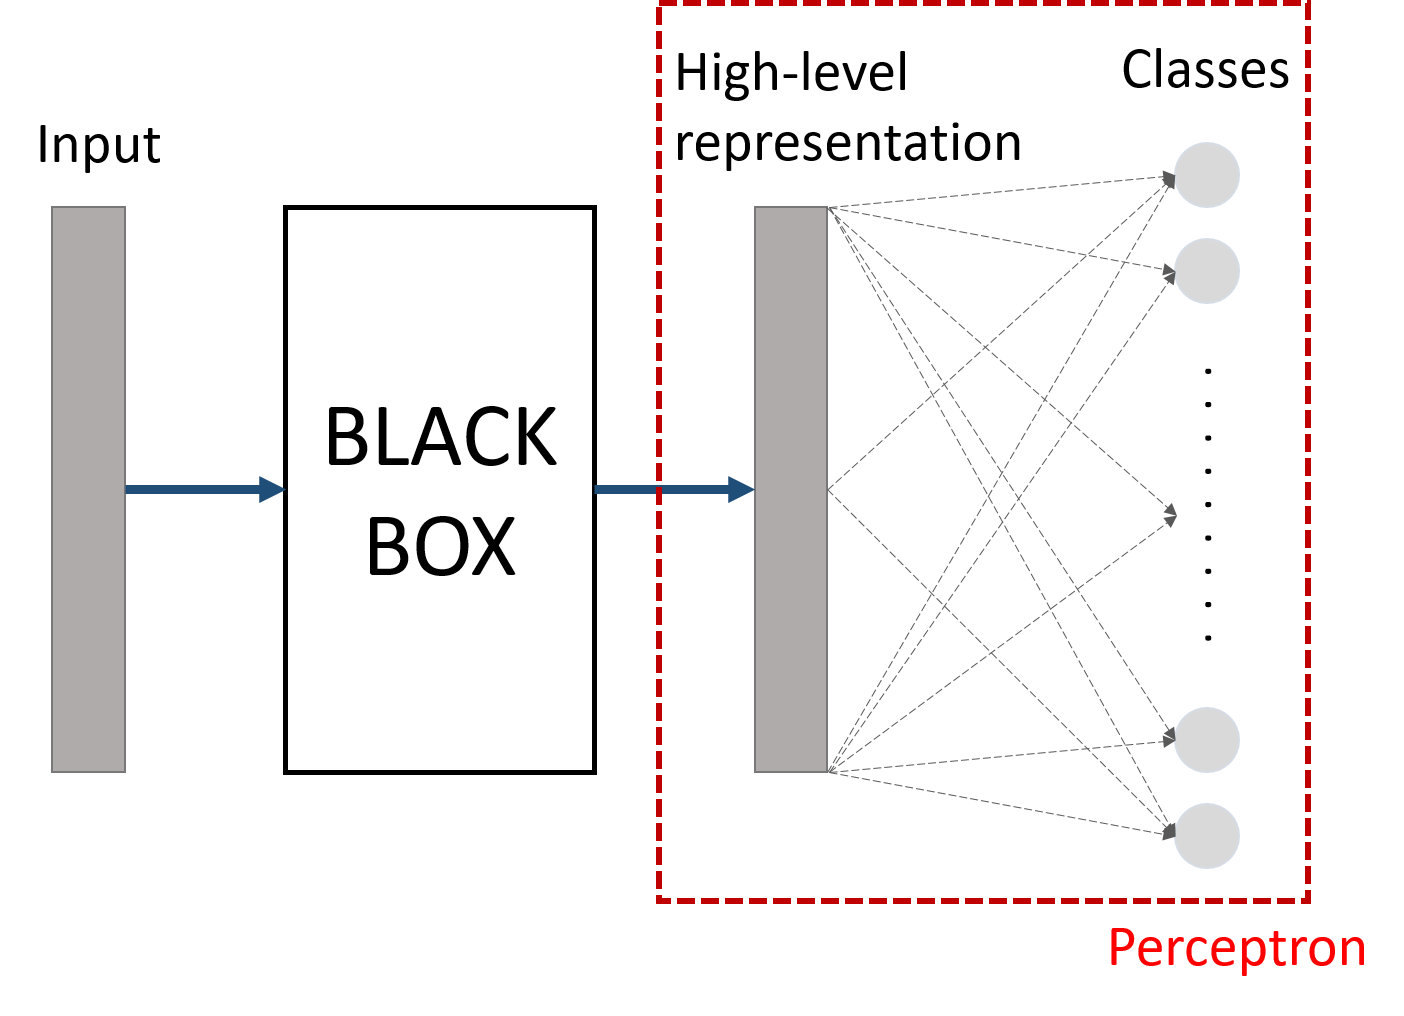
\includegraphics[width=0.85\linewidth]{slides/perceptron_on_top}
  \end{figure}
\end{frame}

\begin{frame}
\frametitle{Results -- Unsupervised Learning with CAE}
  \begin{itemize}
    \item Raw: Perceptron that reads raw input data.
    \item CAE features: Perceptron stacked on the middle layer of the CAE.
    \item CAE architecture: Perceptron stacked on the middle layer of the
      CAE but train the whole network in a supervised way as a CNN.
  \end{itemize}
  \begin{table}[H]
    \tabcolsep = 9pt
    \begin{tabular*}{\linewidth}{>{\bf}llccc}
      \toprule
      && Raw & CAE features & CAE architecture\\
      \midrule
      \multirow{2}{*}{Intensity} &
      train & 69.47 \% & 78.87 \% & 91.29 \% \\
      & test & 32.64 \% & 50.24 \% & 65.44 \% \\
      \midrule
      \multirow{2}{*}{Depth} &
      train & 63.64 \% & 79.61 \% & 88.80 \% \\
      & test & 29.93 \% & 41.64 \% & 55.62 \% \\
      \bottomrule
    \end{tabular*}
  \end{table}
\end{frame}

\subsection{Shared Representation Learning}

\begin{frame}
  \frametitle{Results -- Shared Representation Learning}
  \begin{figure}
    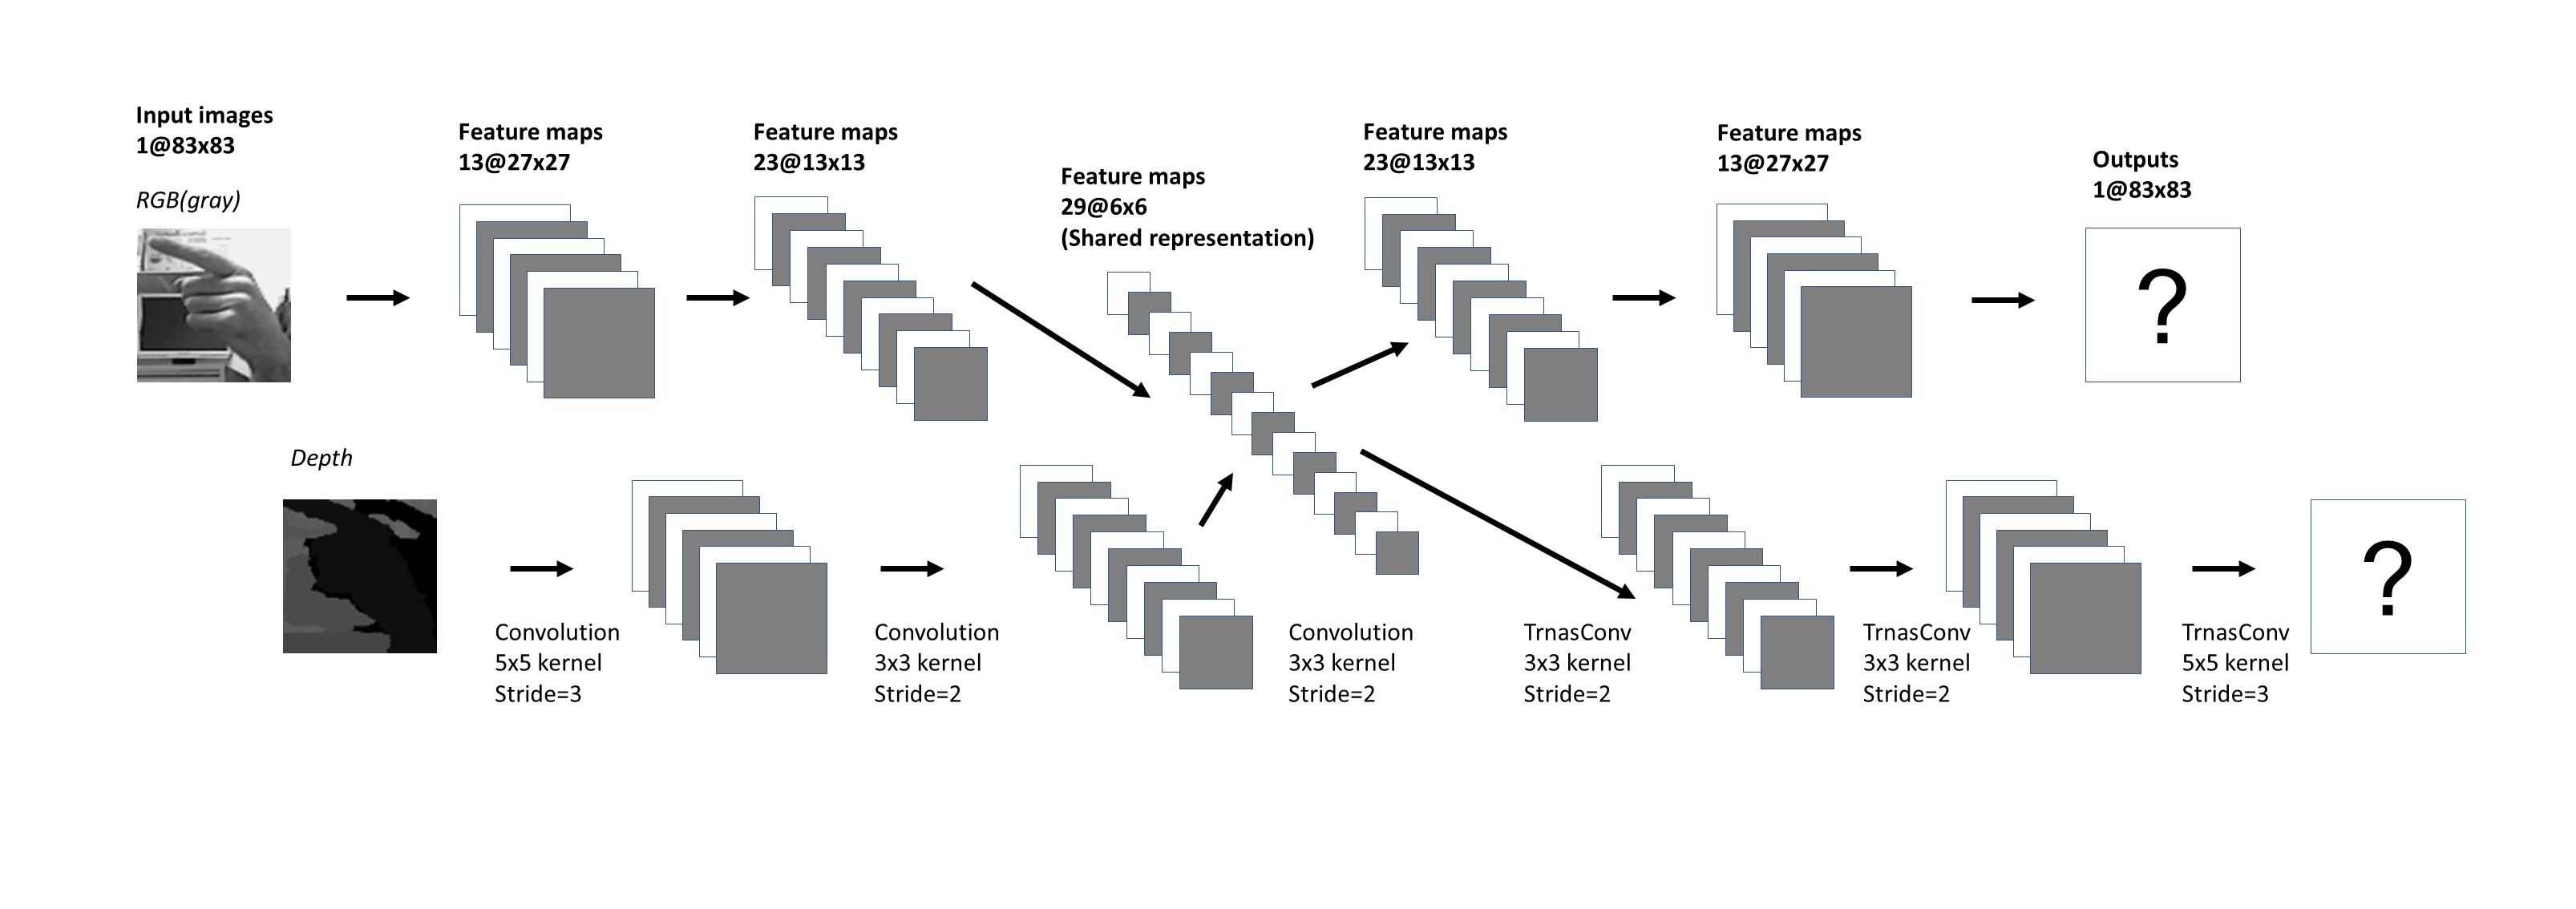
\includegraphics[width=\linewidth]{slides/FAE5}
  \end{figure}
\end{frame}

\begin{frame}
\frametitle{Results -- Shared Representation}
  \begin{itemize}
    \item Shared: Perceptron that exploits the shared representation learned
      by a bimodal CAE.
  \end{itemize}
  \begin{table}[H]
    \tabcolsep = 5pt
    \begin{tabular*}{\linewidth}{>{\bf}llcccc}
      \toprule
      && Raw & CAE features & CAE architecture & Shared\\
      \midrule
      \multirow{2}{*}{Intensity} &
      train & 69.47 \% & 78.87 \% & 91.29 \% & 85.85 \% \\
      & test & 32.64 \% & 50.24 \% & 65.44 \% & 53.38 \% \\
      \midrule
      \multirow{2}{*}{Depth} &
      train & 63.64 \% & 79.61 \% & 88.80 \% & 81.83 \% \\
      & test & 29.93 \% & 41.64 \% & 55.62 \% & 42.85 \% \\
      \bottomrule
    \end{tabular*}
  \end{table}
\end{frame}

\subsection{AVSR Knowledge Transfer}

\begin{frame}
  \frametitle{AVSR Knowledge Transfer}
  \begin{center}
    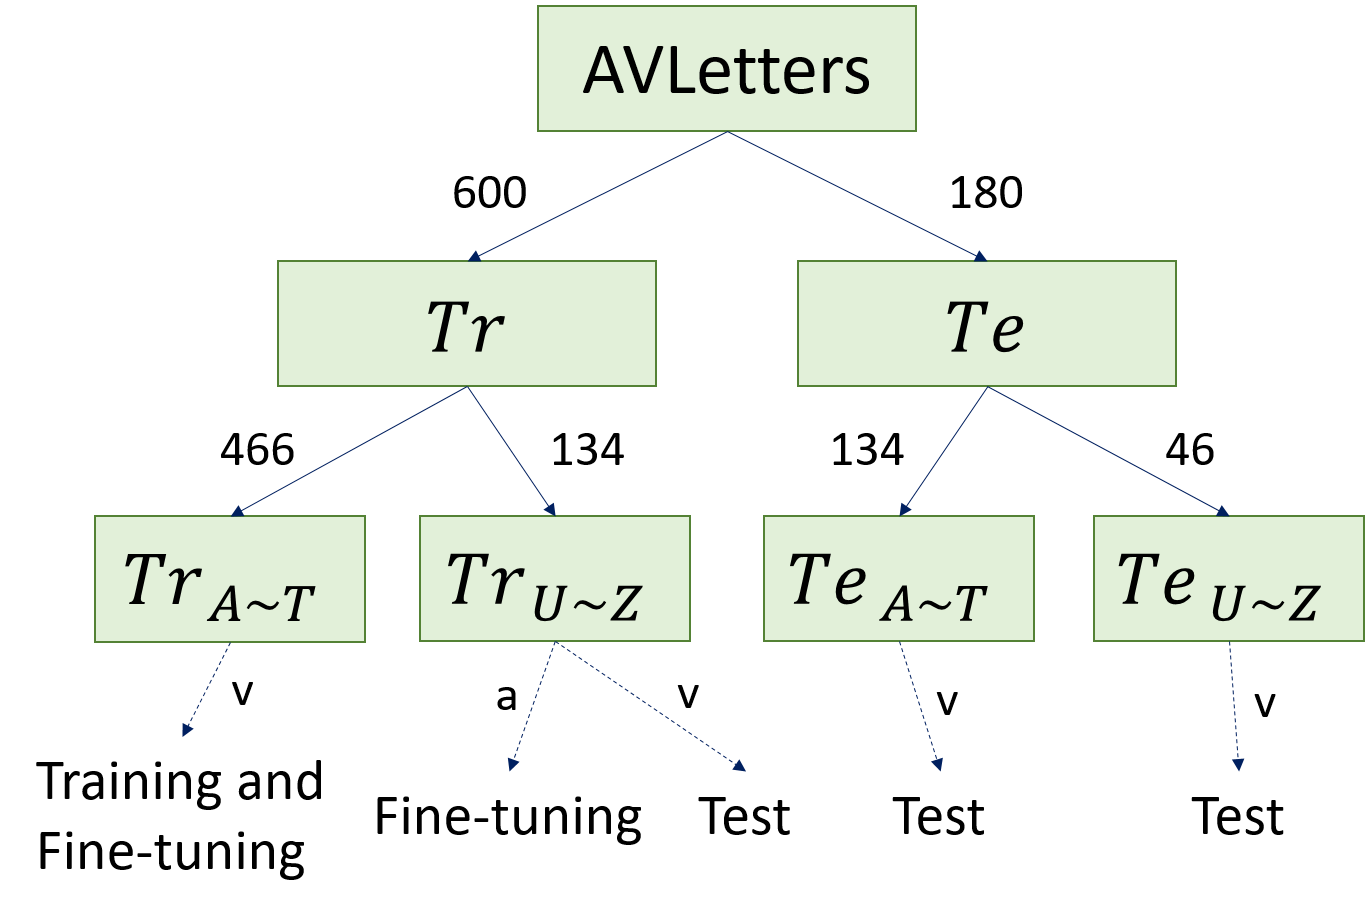
\includegraphics[width=0.83\linewidth]{slides/AVSR_separation}
  \end{center}
\end{frame}

\begin{frame}
  \begin{figure}
    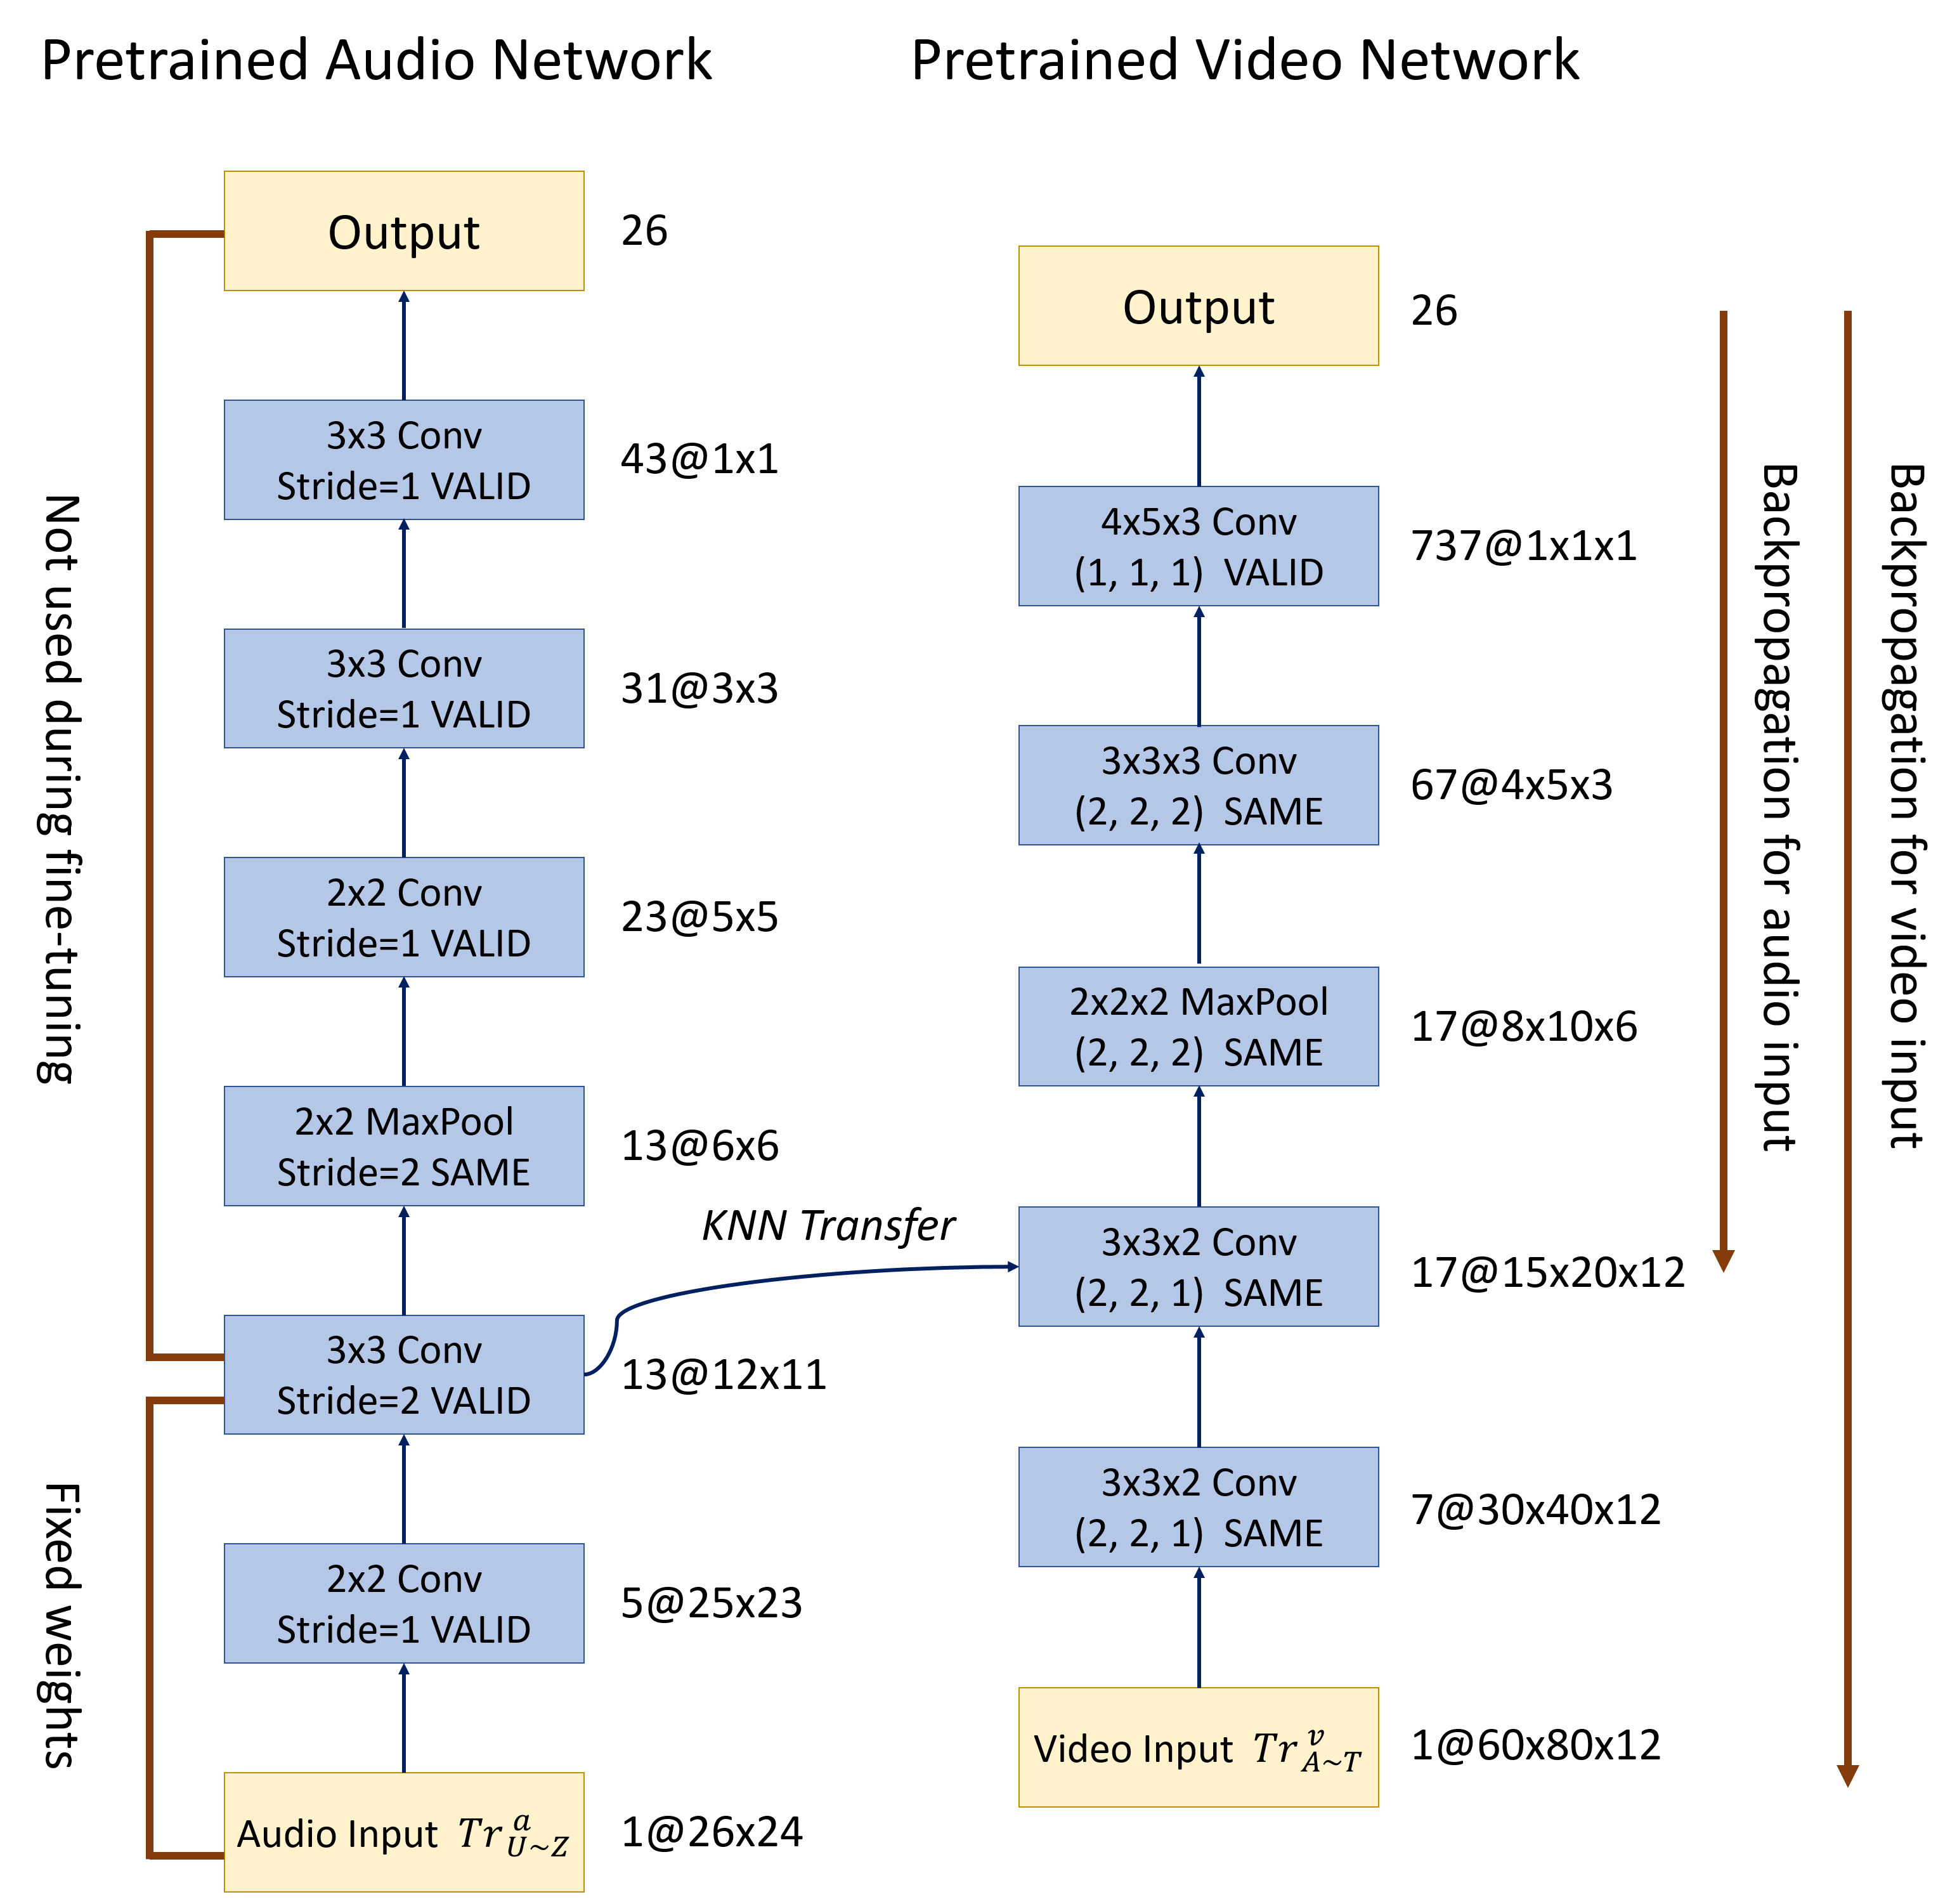
\includegraphics[width=0.75\linewidth]{slides/AVSR_transfer}
  \end{figure}
\end{frame}

\begin{frame}
  \frametitle{AVSR Knowledge Transfer}
    Fine-tuned for 160 steps.\\
    For \textbf{Exp1}, \textbf{Exp2} and \textbf{Exp3}, we have respectively
    $\alpha_0 = 0.001, 0.005, 0.001$ and $p_a = 0.85, 0.85, 1$.\\
    Notice that since $p_a = 1$ for \textbf{Exp3} no video data is given
    in input during fine-tuning.
  \begin{table}[H]
    \tabcolsep = 3pt
    \begin{tabular*}{\linewidth}{>{\bf}lcccccc}
      \toprule
      & $Tr^v$ & $Tr^v_{A\sim T}$ & $Tr^v_{U\sim Z}$
      & $Te^v$ & $Te^v_{A\sim T}$ & $Te^v_{U\sim Z}$\\
      \midrule
      No transfer & 77.67 \% & \textbf{100} \% & 0 \% & \textbf{40.56} \%
      & \textbf{54.48} \% & 0 \% \\
      Exp1 & \textbf{81.17} \% & 98.28 \% & 21.64 \% & 39.44 \%
      & 47.76 \% & 15.22 \% \\
      Exp2 &  40.83 \% & 51.07 \% & 5.22 \% & 23.89 \%
      & 30.60 \% & 4.35 \% \\
      Exp3 & 19.67 \% & 12.23 \% & \textbf{45.52} \% & 12.22 \%
      & 2.24 \% & \textbf{41.34} \% \\
      \bottomrule
    \end{tabular*}
  \end{table}
\end{frame}

\section{Conclusion}

\begin{frame}
  \frametitle{Conclusion}
  \begin{itemize}
    \item Datasets, hyperparameters
    \item Applications in robotics
    \item Other approaches
  \end{itemize}
\end{frame}
